\chapter{The Scope of the Work}
% TODO intro?
\section{The Current Situation}
Der Ist-Zustand der Kundenakquieriung lässt sich anhand der Abbildung \ref{ScopeOfWork:Situation} beschreiben.
\begin{figure}[ht]
  \centering
  % TODO neu in TikZ erstellen
  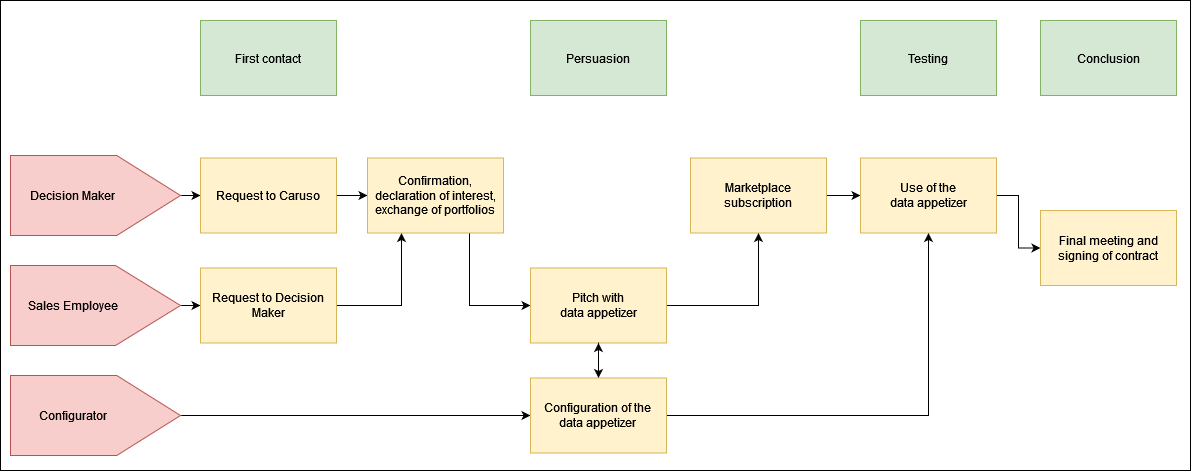
\includegraphics[width=20cm]{scope_of_the_work/current_situation.PNG}
  \caption{Stakeholders}
  \label{ScopeOfWork:Situation}
\end{figure}
Damit ein neuer Vertrag für Caruso zustande kommen kann, werden derzeit drei Stakeholder benötigt, die Entscheidungsträger, die Caruso Sales Mitarbeiter sowie die Caruso Konfiguratoren. Der gesamte Prozess lässt sich in vier Phasen einteilen, die Kontaktaufnahe, die Überzeugungsphase, die Testphase und den Vertragsabschluss.
Zu Beginn befinden sich der Entscheidungsträger und der Sales-Mitarbeiter in der Phase der Kontaktaufnahme. In der Phase fragt der Sales-Mitarbeiter den Entscheidungsträger an, ob Interesse an der Caruso Schnittstelle besteht. Andersherum kann die intiale Anfrage für einen Firmenaustausch auch vom Entscheidungsträger ausgehen. Daraufhin folgt die Zusage beider Stakeholder und ein Termin für ein erstes Treffen wird ausgemacht.

In der Überzeugungsphase präsentiert der Sales Mitarbeiter von Caruso in einem Pitch die visualiserten Daten von vorherigen Fahrzeugen bei Caruso. Dafür erhält der Sales Mitarbeiter derzeit HTML oder Excel-Berichte mit aggergierten Fahrzeuginformationen vergangener Fahrten vom Konfigurator. Dieser stellt die Informationen manuelle bereit, indem er Daten aus vergangen Fahrten aus deinem Zeitraum sammelt und zusammenfasst. Solche Daten sind beispielsweise die Anzahl der gefahrenen Kilometer pro Wochentag über eine gesamte Flotte von Autos.

Nach dem Sales Pitch ist der vertraut der Entscheidungsträger der Schnittstelle von Caruso, sodass er seine eignen Fahrzeuge beim Caruso Marketplace hinzufügen will. Dafür durchläuft er den Prozess der Marketplace Subscription und kann in der Testphase nach ein bis zwei Wochen aggregierte Fahrzeuginformationen vom Konfigurator erhalten. Dies beinhaltet in der Regel keine Live-Informationen.
Sobald der Kunde von überzeugt ist, klärt er offene Fragen mit dem Sales-Mitarbeiter in einem Abschlussgespräch ab und es kommt daraufhin zum Vertragsabschluss.

\section{The Context of the Work}
Figure \ref*{ScopeOfWork:ContextDiagram} shows the communication between the core target group, the Carvis and the neighbouring systems in the form of a context diagram.

% TODO in TikZ neu erstellen
% TODO Konfigurator unter Sales Employee
\begin{figure}[ht]
  \centering
  \includegraphics*[width=10cm]{./context_diagram.png}
  \caption{Context Diagram}
  \label{ScopeOfWork:ContextDiagram}
\end{figure}

The Decision Maker has access to both the Caruso Marketplace and Carvis. The access to the Marketplace is required as the Decision Maker needs to create an account and register vehicles before they can access Carvis.

The Sales Employee uses Carvis to present Caruso Data to the Decision Maker. They are not allowed to access the Decision Makers data but can use placeholder cars publically accessible in the Caruso Marketplace.

The Configurator only needs access to Carvis in order to configure it for the Sales Employee.

Both systems get their data from the Caruso API which recieves live data from the OEMs and standardizes it.
% TODO ausformulieren?